\documentclass{article}
\usepackage[dvipsnames,table]{xcolor}
\usepackage[portuguese]{babel}
\usepackage[utf8x]{inputenc}
\usepackage[T1]{fontenc}
\usepackage{amsmath}
\usepackage{graphicx}
\usepackage{float}
\usepackage[colorinlistoftodos]{todonotes}
\usepackage{titling}
\usepackage{natbib}
\setcitestyle{square}
\usepackage{mathtools}
\usepackage{empheq}
\usepackage{tensor}
\usepackage{microtype}
\usepackage{listings}
\usepackage[all]{xy}
\usepackage[labelformat=empty]{caption}
\usepackage{indentfirst}
\usepackage[dvipsnames]{xcolor}
\usepackage{alloy-style}
\newcommand\tab[1][1cm]{\hspace*{#1}}
\definecolor{someGray}{RGB}{230,230,230}
\usepackage{hyperref}
\newcommand{\subtitle}[1]{%
  \posttitle{%
    \par\end{center}
    \begin{center}\large#1\end{center}
    \vskip0.5em}%
}


\begin{document}


\title{Modelação Formal de um sistema de suporte a uma ontologia de TS-RADA para a Plataforma M-51-CLAV}
\subtitle{Mestrado Integrado em Engenharia Informática \\ Laboratório de Engenharia Informática \\ 4º Ano, 2º Semestre}
\author{A82441 - Alexandre Pinho \and A82313 - Pedro Gonçalves} 

\begin{figure}
\centering

\includegraphics[scale=1.5]{images/logoUM.png}
\end{figure}
\par
\date{Braga, julho de 2020}

\maketitle


% necessário?
%\begin{abstract}
%\end{abstract}

\thispagestyle{empty}
\newpage
\setcounter{page}{1}
\tableofcontents
\newpage
\listoffigures
\newpage


%\begin{figure}[H]
%    \begin{centering}
%         \centerline{\frame{\includegraphics[width=\linewidth]{images/Automato.jpg}}}
%         \captionof{figure}[Autómato Temporal Aventureiro]{Figura 1 - Autómato Temporal Aventureiro.}
%    \end{centering}
%\end{figure}

\section{Introdução}

% contextualização: administração governamental produz muita informação, que precisa de ser catalogada e tratada
A Administração Pública, as empresas públicas e entidades relacionadas com o Estado produzem, hoje em dia, uma quantidade e diversidade de informação impossíveis de organizar e processar sem recurso a sistemas digitais de informação.

% plataforma CLAV, PGDs, e RADAs; objetivo do trabalho
Para esse propósito, foi desenvolvida a plataforma CLAV:

\begin{quote}
    A CLAV é uma Plataforma desenvolvida pela Direção-Geral do Livro, dos Arquivos e das Bibliotecas, que disponibiliza a «Lista Consolidada para a classificação e avaliação da informação pública» enquanto instrumento facilitador da elaboração dos planos de classificação e tabelas de seleção da Administração Pública, de empresas públicas e de outras entidades\cite{clav}.
\end{quote}

O sistema funciona através da utilização de uma linguagem comum para a avaliação dos documentos e especificação da sua informação arquivística, e do estabelecimento de uma Portaria de Gestão de Documentos (PGD) em cada entidade que irá integrar a Lista Consolidada. No entanto, existe já documentação acumulada que não pode ser processada pelas PGDs. Para classificar e avaliar esta documentação, foi desenvolvido um novo instrumento, o Relatório de Avaliação de Documentação Acumulada (RADA). Assim, é proposto proceder à modelação formal do sistema de suporte à ontologia da plataforma CLAV envolvendo o conceito de RADA.

% estrutura do relatório
Nas próximas páginas, é feita a modelação formal do modelo, a sua correspondente modelação em Alloy, é construída uma ontologia OWL com recurso à ferramenta \emph{Protégé}, são indicadas as dificuldades enfrentadas ao longo do desenvolvimento do projeto, e, por fim, retiram-se as conclusões e identificam-se as áreas de trabalho futuro.

\newpage
\section{Modelação formal} 

\par Neste capítulo vai ser discutida a abordagem levada a cabo pelo grupo durante o processo de especificação do modelo formal. Para tal, foi analisado um documento, desenvolvido pelo Professor José Carlos Ramalho, onde estavam descritos os requisitos necessários para o bom funcionamento do RADA. Tendo por base esse documento, foi então possível perceber quais as entidades, as suas relações e os invariantes necessários para a criação de um modelo formal do RADA. %Falta colocar o documento nas referências e colocar a citação aqui
\par Os resultados desta análise estão descritos nos sub-capítulos seguintes.

\subsection{Identificação de entidades}
% entidades relevantes ao âmbito do trabalho

\par Devido ao âmbito limitado do projeto, nem todas as entidades de um eventual modelo completo da plataforma CLAV foram incluídas no modelo concebido, sendo apenas modelado as entidades pertencentes ao TS-RADA. Assim, foram identificadas as seguintes entidades:

\begin{itemize}
    \item Relatório de Avaliação de Documentação Acumulada (RADA)
    \item Relatório Expositivo do RADA
    \item Tabela de Seleção
    \item Prazo de Conservação Administrativa (PCA)
    \item Destino Final (DF)
    \item Justificação
        \par \tab Justificação para PCA ou DF
    \item Critério
        \par \tab Critério de justificação, com possíveis valores \texttt{Critério de utilidade administrativa}, \texttt{Critério de complementaridade informacional}, \texttt{Critério de densidade informacional}, \texttt{Critério legal}, \texttt{Critério gestionário}.
    \item Classe N1
    \item Classe N2
    \item Classe N3
    \item Classe de Série
    \item Classe de Subsérie
    \item Unidade de Instalação (UI)
    \item Entidade
        \par \tab Entidades públicas que intervêm nos processos de negócio (classes de 3º nível) da Lista Consolidada.
    \item Tipologia de Entidade
        \par \tab Forma de agrupamento de entidades que intervêm nos processos de negócio (classes de 3º nível) da Lista Consolidada.
    \item Legislação
    \item Auto de Eliminação
\end{itemize}

\subsection{Identificação de relações}
% relações entre essas entidades, incluindo multiplicidade
% relações inversas e simétricas

\par Já no capítulo das relações entre as diferentes entidades, foram encontradas 95 relações. Depois de identificadas todas estas relações, é necessário classificar as mesmas relativamente à sua multiplicidade, ou seja, perceber se as relações são simples, inteiras, injetivas e/ou subjetivas. Por fim, é preciso compreender como as mesmas se relacionam entre si, isto é, proceder à identificação das relações inversas/conversas e simétricas entre si.

\par Os seguintes diagramas relacionais representam graficamente de uma forma simplificada as principais relações do sistema a modelar.
\par Este primeiro diagrama, representa de uma forma muito simples, as principais entidades do RADA, e algumas relações entre as mesmas. Como podemos observar, Entidades relacionam-se de forma direta com Autos de Eliminação, RADAs e Relatórios Expositivos. Já os RADAS relacionam-se com Autos de Eliminação e Relatórios Expositivos, mas também com Tabelas de Seleção, que por sua vez se relacionam com Classes.
\begin{equation}
    \xymatrix{
    & & & Entidade \ar[dd]|{eResponsavelPor} \ar[ddlll]_{prodDocAvaliadaPor} \ar[ddrrr]^{prodDocAvaliadaPor} \\ \\
    AE \ar[dd]|{referencia} & & & RADA \ar[lll]_{avaliaDocEliminadaPor}  \ar[dd]|{contemTS} \ar[rrr]^{contemRE} & & & RE \\ \\
    Classe & & & TSRada \ar[lll]_{temClasse} \\
    }
\end{equation}

\par Já no diagrama em baixo está representada, também de forma simplificada, a hierarquia existente entre os diferentes tipos de Classes. 
\begin{equation}
    \xymatrix{
        ClasseN1 \ar[dd]|{ePaiDeN2} \\ \\
        ClasseN2 \ar[dd]|{ePaiDeN3} & & &
            ClasseSerie \ar[uulll]_{eFilhaDeN1}
                        \ar[lll]^{eFilhaDeN2}
                        \ar[ddlll]^{eFilhaDeN3}
                        \ar[rrr]^{ePaiDeSubSerie}  & & & ClasseSubSerie\\ \\
        ClasseN3
    }
\end{equation}

\subsection{Identificação de invariantes}
% invariantes sobre as entidades e relações (não específicos ao Alloy)

\par A fase final deste processo de especificação do modelo formal, consiste em identificar as propriedades necessárias garantir para garantir o correto funcionamento do RADA, ou seja identificar os invariantes do sistema. Assim sendo, além da análise ao documento, foi necessário reunir com o Professor José Carlos Ramalho para conseguir identificar todas as propriedades, pois o documento não referia a totalidade dos invariantes.
\par Posto isto, foram identificados perto de 30 invariantes, sendo que os podemos dividir em duas categorias. A primeira categoria, corresponde aos invariantes que dizem respeito à parte semântica/funcional do RADA, sendo que a segunda corresponde à taxonomia das relações.
%Talvez também dar um exemplo usando a notação do jno?

\newpage
\section{Modelação em Alloy}
% breve explicação do Alloy
% (modelo completo em anexo)

\par Depois de concluído o processo de especificação do modelo formal, descrito no capítulo anterior, é necessário verificar a existência de instâncias capazes de habitarem esse modelo. Para isso são usadas ferramentas de \emph{model checking}, visto que fazem a geração/verificação de instâncias de forma automática. Assim sendo, para este projeto foi usado o Alloy Analyser para proceder à verificação das propriedades do modelo.
\par Na figura 1, é apresentada uma instância do RADA gerada pela ferramenta Alloy.

%Colocar instância gerado pelo alloy
\begin{figure}[H]
    \begin{centering}
         \centerline{\frame{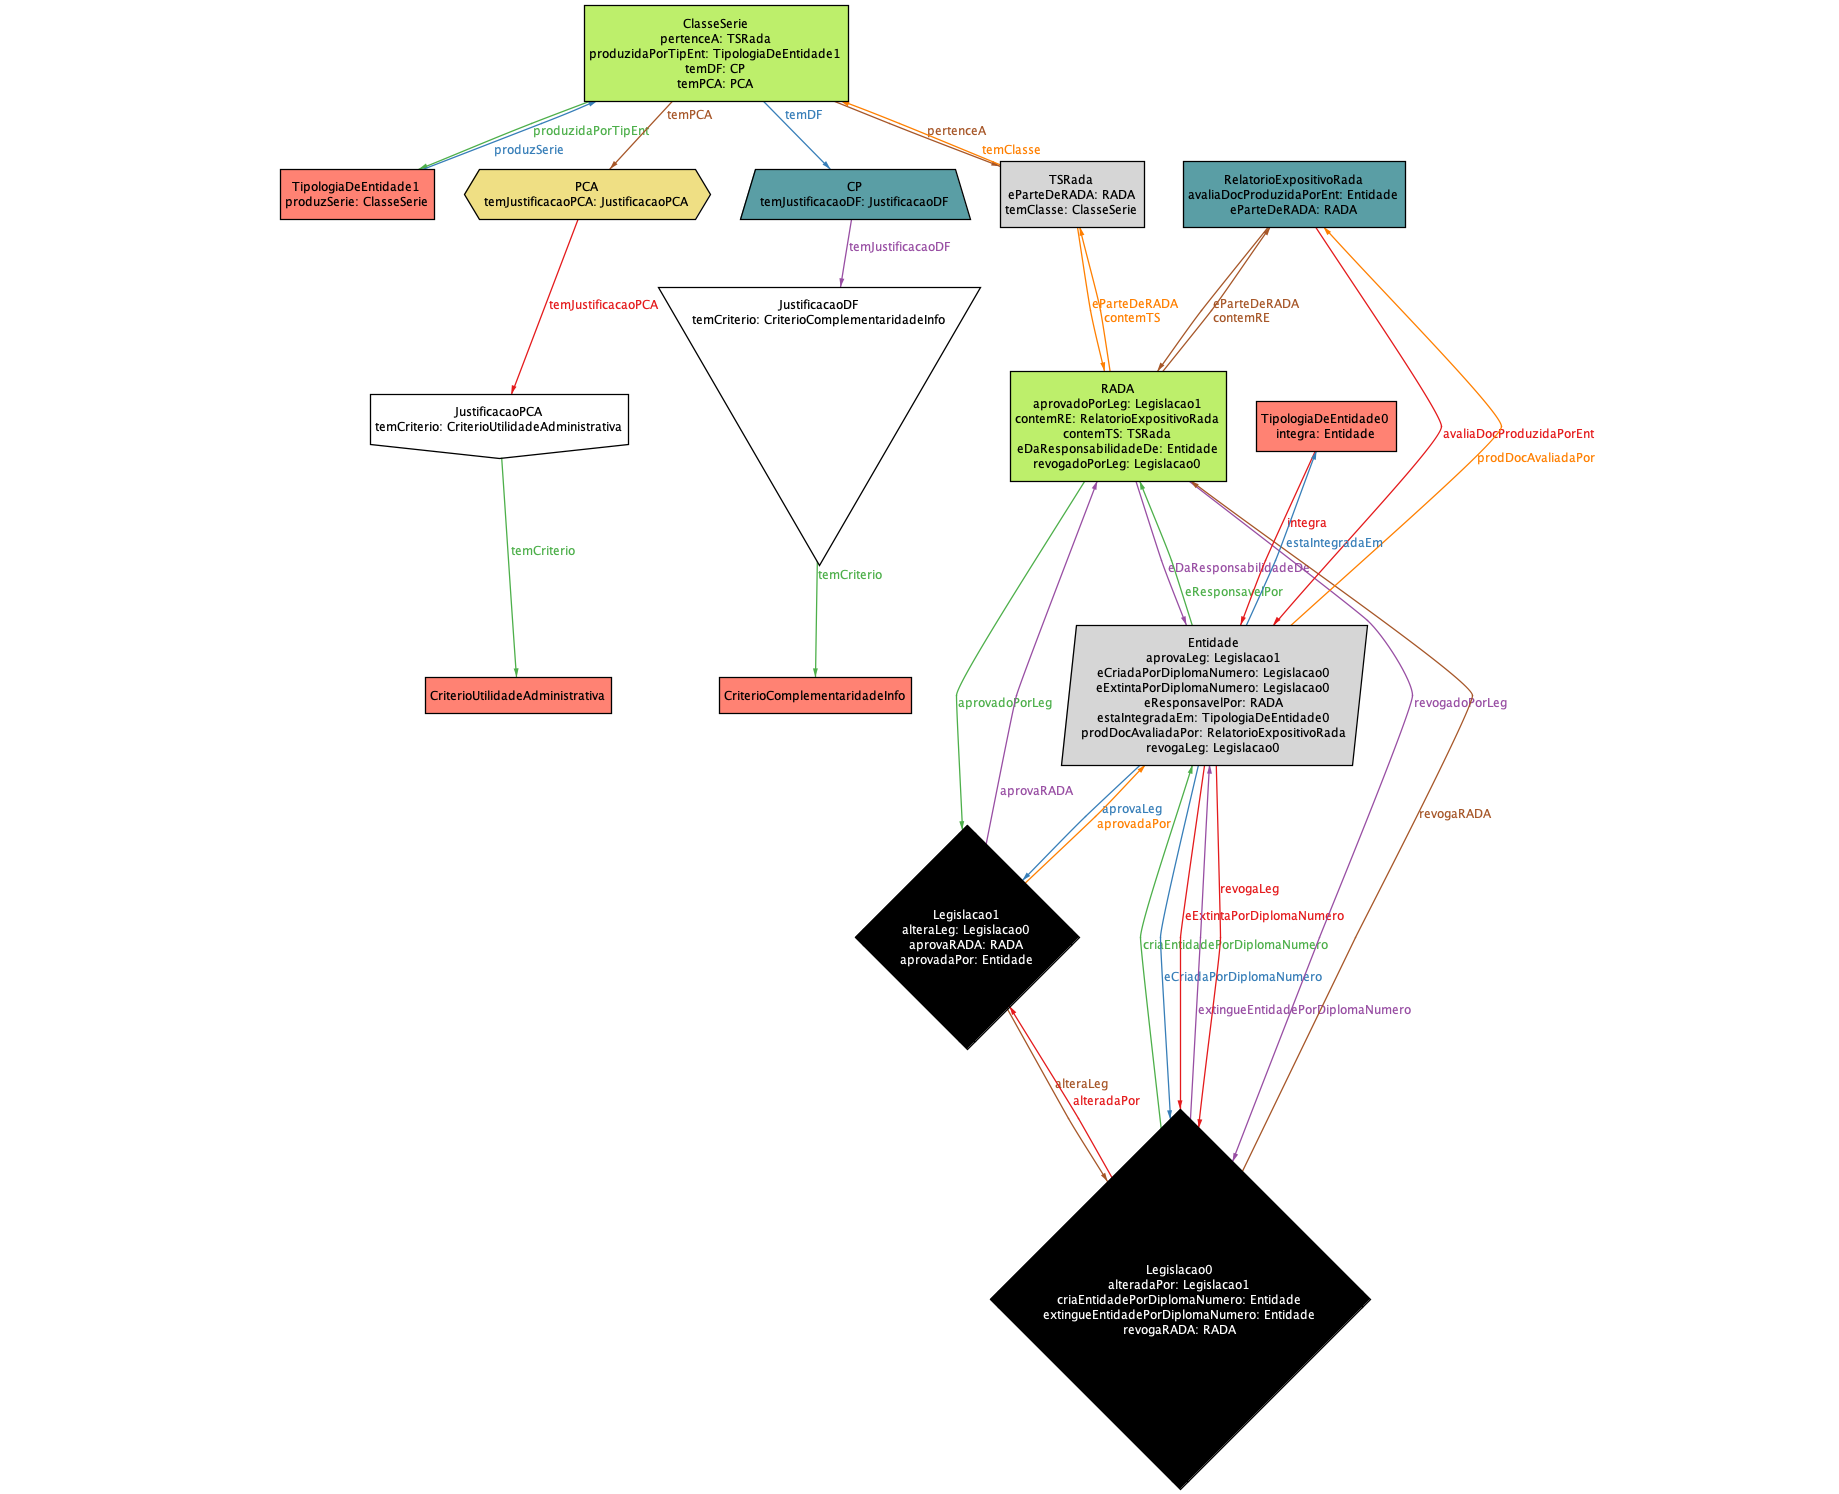
\includegraphics[scale=0.25]{images/InstanciaAlloy.png}}}
         \captionof{figure}[Instância do modelo gerada na ferramenta Alloy]{Figura 1 - Instância do modelo gerada na ferramenta Alloy.}
    \end{centering}
\end{figure}

\par Nesta secção, vai ser abordada a forma como foi feita a tradução do modelo formal para um modelo Alloy. O resultado dessa tradução encontra-se no anexo \ref{appendix:A} deste relatório.


\subsection{Especificação}
% explicar como os vários conceitos foram modelados em Alloy (exemplificando):
% - entidades -> sigs
% - relações idênticas de entidades relacionadas (ClasseN1/2/3, Criterio(...)) -> relações em sigs abstratas + sigs com keyword 'extends'; etc.
% - relações inversas (e simétricas) -> ~R = S, ou no caso de relações com o mesmo nome mas domínios e/ou contra-domínios diferentes ~(D <: R) = S :> CD) (restrição de domínio/contra-domínio)

\par A primeira parte da tradução de um modelo formal para um modelo Alloy, consiste na correspondência das entidades para primitivas \emph{sig} em Alloy. Já a noção de herança de propriedades entre as diferentes entidades é representada em Alloy, usando as primitivas \emph{abstract} e \emph{extends}, baseadas nos conceitos de programação orientada a objetos. Em baixo é apresentado um excerto do modelo onde se podem verificar exemplos dessas traduções.

\begin{lstlisting}[language=alloy, frame=single]
abstract sig Criterio{}

sig CriterioGestionario extends Criterio{
}
\end{lstlisting}

\par Para o caso das relações entre entidades, essas são representadas da seguinte forma:

\begin{lstlisting}[language=alloy, frame=single]
sig TSRada {
	eParteDeRADA : one RADA,
	temClasse : set Classe
}
\end{lstlisting}

\par Como se pode observar, estão definidas duas relações no excerto acima. A primeira relação, eParteDeRada, possui cardinalidade \emph{one} no contradomínio, ou seja é uma relação de 1 TSRada para 1 RADA. Já a segunda relação, temClasse, possui cardinalidade \emph{set}, o que significa que para cada TSRada está relacionado com 0 ou mais Classes. 
% Colocar setas das relações em baixo no texto
%TSRada \xleftarrow[]{\text{eParteDeRada}} RADA\_N1$
%TSRada \xleftarrow[]{\text{temClasse}} Classe\_N1$

\par Por fim, outro aspeto importante da tradução para um modelo Alloy, é a definição de relações inversas e de relações com o mesmo nome, mas com domínios/contra-domínios diferentes. A tradução deste tipo de casos é exemplificado no exemplo a seguir.

\begin{lstlisting}[language=alloy, frame=single]
temSucessor = ~temAntecessor

ClasseSerie <: ePaiDeUI = ~eFilhoDeSerie
ClasseSubSerie <: ePaiDeUI = ~eFilhoDeSubSerie
\end{lstlisting}

\par Como se pode observar no excerto em cima, a forma como se define uma relação inversa em Alloy é utilizando o caracter til, ou seja, é possível observar que relação temSucessor é inversa da relação temAntecessor. Já as outras duas expressões, representam a forma de como é possível restringir, neste caso o domínio, para o caso de relações que possuem mais que um inverso, como é o caso da relação ePaiDeUI.

\subsection{Verificação}
\par Depois de traduzido o modelo formal para a linguagem do Alloy, é possível utilizar lógica de primeira ordem para especificar os invariantes, de modo a ser possível verificar se os mesmos criam inconsistências no sistema.
\par Vamos agora apresentar alguns exemplos de tradução direta de invariantes para Alloy, e também um exemplo de um invariante que foi criado apenas com o objetivo de garantir que a instância criada pelo Alloy representa de forma correta o modelo formal.

\begin{lstlisting}[language=alloy, frame=single]
all A : ClasseSerie | no A.eSinteseDeSerie & A.eSintetizadaPorSerie
all A : ClasseSubSerie | no A.eSinteseDeSubSerie & A.eSintetizadaPorSubSerie

all A, B : ClasseSerie | (
    B in A.eSintetizadaPorSerie implies (
        A.temDF in Eliminacao
    )
)
all A : ClasseSubSerie, B : ClasseSubSerie | (
    B in A.eSintetizadaPorSubSerie implies (
        A.temDF in Eliminacao
    )
)
\end{lstlisting}
\par Estes invariantes apresentados em cima, representam uma tradução direta de invariantes identificados pelo modelo formal, utilizando lógica de primeira ordem. Os invariantes utilizados neste exemplo correspondem, respetivamente, ao invariantes 3 e 4 do modelo Alloy apresentado no anexo \ref{appendix:A} deste relatório.

\begin{lstlisting}[language=alloy, frame=single]
all j:JustificacaoDF | j in DF.temJustificacaoDF
all j:JustificacaoPCA | j in PCA.temJustificacaoPCA
all df:DF | df in (ClasseSerie.temDF + ClasseSubSerie.temDF)
all pca:PCA | pca in (ClasseSerie.temPCA + ClasseSubSerie.temPCA)
all c:Criterio | c  in Justificacao.temCriterio
\end{lstlisting}
\par Já este segundo conjunto de invariantes serve apenas para garantir que nas instâncias criadas pelo modelo Alloy, não apareçam entidades isoladas no modelo, ou seja não é um invariante do modelo formal propriemente dito, mas sim do Alloy.

% - invariantes identificados -> linguagem do Alloy (dar dois ou três exemplos distintos)
% - invariantes específicos ao Alloy (exemplo: verificar que todas as entidades têm pelo menos uma relacão com outra entidade)

\newpage
\section{Ontologia OWL}
% explicar a transformação do modelo em Alloy para a ontologia OWL
% - sigs -> hierarquia de classes
% - ...

Por fim, é desenvolvida a ontologia OWL com recurso à ferramenta \textit{Protégé}. Uma ontologia OWL consiste nos conjuntos de classes, propriedades de objetos, e propriedades de dados definidos.

Nesta secção, serão explicados os métodos utilizados para construir a ontologia RADA.

\subsection{Definição de classes}

As classes de objetos definidas são os conjuntos de indivíduos que representam os conceitos do modelo. Para o modelo em questão, são definidas treze classes nomeadas representando os conceitos principais, e adicionalmente mais dez classes nomeadas que são subclasses das classes de topo nível, pois representam diferentes categorias dessa classe, como, por exemplo, na classe \texttt{Criterio}. A hierarquia de classes é apresentada a seguir, sendo que a indentação indica a sua estrutura:

\begin{verbatim}
owl:Thing
        AutoDeEliminacao
        Classe
                ClasseN1
                ClasseN2
                ClasseN3
                ClasseSerie
                ClasseSubSerie
        Criterio
                CriterioComplementaridadeInfo
                CriterioDensidadeInformacional
                CriterioGestionario
                CriterioLegal
                CriterioUtilidadeAdministrativa
        DF
                CP
                Conservacao
                Eliminacao
        Entidade
        Justificacao
                JustificacaoDF
                JustificacaoPCA
        Legislacao
        PCA
        RADA
        RelatorioExpositivoRada
        TSRada
        TipologiaDeEntidade
        UI
\end{verbatim}

Todas as classes que são subclasses da mesma classe são definidas como disjuntas, significando que um indivíduos não pode pertencer a mais que uma classe nesta ontologia.

\subsection{Definição de propriedades de objetos}

De seguida, são definidas as propriedades de objetos, ou seja, as relações entre indivíduos das classes. Para a maior parte destas propriedades, apenas é necessário defini-la como uma propriedade de topo nível, especificar o seu domínio e contra-domínio, indicar, se existir, a sua propriedade inversa, e indicar se representa uma relação simples ("Functional" no \emph{Protégé}), e no caso das propriedades \texttt{eComplementar} e \texttt{eCruzado} indicar que se trata de uma propriedade simétrica.

No entanto, nem todas as propriedades têm apenas indivíduos de uma classe como o seu domínio ou contra-domínio, dificultando a sua modelação. Através da construção de uma hierarquia de propriedades para cada uma destas, é possível modelar relações com nomes iguais e domínios distintos. Por exemplo, o domínio da relação \texttt{ePaiDeSerie} é a união das classes \texttt{ClasseN1}, \texttt{ClasseN2} e \texttt{ClasseN3}; então, é necessário criar as duas seguintes hierarquias de classes:

\begin{verbatim}
Classe_ePaiDeSerie
        ePaiDeSerieClasseN1
        ePaiDeSerieClasseN2
        ePaiDeSerieClasseN3

eFilhaDe
        eFilhaDeN1
        eFilhaDeN2
        eFilhaDeN3
\end{verbatim}

Assim, as propriedades \texttt{Classe\_ePaiDeSerie} e \texttt{eFilhaDe} têm, respetivamente, domínio e contra-domínio de \texttt{ClasseN1 or ClasseN2 or ClasseN3}, são inversas entre si, e as subpropriedades têm domínios e contra-domínios de apenas uma das classes, e são também inversas entre si.

\subsection{Definição de restrições}

As restrições descrevem classes que se definem pelas relações em que os seus indivíduos participam. Ao estabelecer a equivalência estas classes com as classes que representam os conceitos na ontologia, é possível verificar que todos os indivíduos que fazem parte da classe respeitam certas regras, e vice-versa.

São definidas nove restrições em oito classes para a especificação de multiplicidade de relações, de duas formas: quando a relação é uma função (simples e inteira), utiliza-se a restrição \texttt{R exactly 1 A}; e quando a relação é não é vazia, a restrição utilizada tem o formato \texttt{R some A}. São estas todas as restrições definidas:

\begin{verbatim}
(AutoDeEliminacao) legitimadoPor exactly 1 Legislacao
(Classe) pertenceA exactly 1 TSRada
(ClasseN2) eFilhoDeN1 exactly 1 ClasseN1
(ClasseN3) eFilhoDeN2 exactly 1 ClasseN2
(DF) temJustificacaoDF exactly 1 JustificacaoDF
(Entidade) eCriadaPorDiplomaNumero exactly 1 Legislacao
(Entidade) eExtintaPorDiplomaNumero exactly 1 Legislacao
(Justificacao) temCriterio some Criterio
(PCA) temJustificacaoPCA exactly 1 JustificacaoPCA 
\end{verbatim}

\subsection{Definição de propriedades de dados}

Para completar o modelo, são definidas as propriedades de dados, que são as propriedades usadas para associar dados de um determinado tipo (contra-domínio) a indivíduos de certas classes. Como no caso das propriedades de objetos com nomes iguais, é criada um hierarquia de propriedades de dados para lidar com propriedades de diferentes classes com o mesmo nome, por exemplo, as propriedades "código" ou "descrição".


% talvez em anexo isto?
São utilizados os seguintes critérios para definir os contra-domínios das propriedades, que representam o tipo de dados utilizados:

\begin{itemize}
    \item Códigos de identificação (inc. propriedades "identificador"): \texttt{xsd:token}
    \item Datas: \texttt{xsd:dateTime}
    \item Descrições, títulos, nomes, e notas: \texttt{xsd:string}
    \item Propriedade "estado": \texttt{xsd:boolean}
    \item Propriedade "estadoDeConservação": \texttt{xsd:string}
    \item Propriedade "formaContagemPCA": \texttt{xsd:float}
    \item Propriedades "historiaAdministrativaBiografica" e "historiaCustodial": \texttt{xsd:string}
    \item Propriedade "internacional": \texttt{xsd:boolean}
    \item Propriedade "link": \texttt{xsd:anyURI}
    \item Localizações: \texttt{xsd:string}
    \item Propriedade "medição": \texttt{xsd:string}
    \item Propriedades "mediçãoDasUIEmDigital" e "mediçãoDasUIEmPapel": \texttt{xsd:float}
    \item Propriedades "mediçãoDasUINoutrosSuporters": \texttt{xsd:string}
    \item Propriedade "número": \texttt{xsd:integer}
    \item Propriedade "númeroDeDiploma": \texttt{xsd:token}
    \item Propriedades "númeroDeUI" e "numeroDeAuto": \texttt{xsd:int}
    \item Propriedade "PCA": \texttt{xsd:float}
    \item Propriedade "serieAbertaFechada": \texttt{xsd:boolean}
    \item Propriedade "sigla": \texttt{xsd:token}
    \item Propriedade "sistemaDeOrganização": \texttt{xsd:string}
    \item Propriedade "sumario": \texttt{xsd:string}
    \item Propriedade "suporte": \texttt{xsd:string}
    \item Propriedade "tipoDeDiploma": \texttt{xsd:string}
    \item Propriedade "tipoDeUnidadeArquivistica": \texttt{xsd:string}
\end{itemize}

\newpage
\section{Dificuldades}
% dificuldades
% - Fucking covid-19
% - relações com nomes iguais mas domínios e contra-domínios diferentes

\par Durante o desenvolvimento deste projeto foram surgindo algumas dificuldades que tiveram impacto no progresso do trabalho.
\par A principal dificuldade surgiu devido à pandemia mundial de Covid-19, que além de atrasar o desenvolvimento do projeto devido à interrupção letiva que provocou, dificultou o processo de reuniões com o coordenador do projeto. Outro aspecto que afetou este projeto foi o aumento da carga de trabalho nas outras unidades curriculares, devido também à pandemia, o que deixou os alunos com menos horas para a realização do mesmo.
\par Outra dificuldade que o grupo encontrou, esta relativa ao desenvolvimento do modelo OWL, foi o facto de existirem relações com nomes iguais mas com domínios/contra-domínios diferentes, o que originou umas complicações na construção do modelo OWL, comparativamente ao modelo Alloy.

\newpage
\section{Conclusão e Trabalho Futuro}
% conclusão
% - modelação parcial do sistema em Alloy
% - desenvolvida um ontologia de parte do sistema da plataforma CLAV
% - (?) foram/não foram encontradas inconsistências nos requisitos para a elaboração dos RADA (perguntar ao stor?) - Segundo os nossos modelos não existem inconsistências
% - ...

% trabalho futuro:
% - modelar mais aspetos do problema, como as datas dos prazos e invariantes relacionados
% - formar queries SPARQL a partir dos invariantes

\par Fazendo uma retrospectiva a todo o trabalho desenvolvido, o grupo pode afirmar que este foi concluído com sucesso, pois foram alcançados todos os objetivos propostos no início do semestre, que eram a formalização e verificação do modelo formal, e ainda foi possível fazer algum trabalho extra na formalização do modelo OWL. %adicionar depois link para o github do projeto
\par Com o trabalho desenvolvido na formalização e verificação do modelo formal, foi possível verificar que o modelo desenvolvido não possui inconsistências, o que era um dos objetivos no início do projeto.
\par O modelo formal apresentado em anexo consiste apenas na formalização da parte relativa ao RADA. Na realidade, o CLAV possui outros componentes que interagem entre si, e seria bom verificar que todos esses componentes funcionam da maneira correta. Sendo assim, um trabalho futuro passaria por verificar de modo formal os restantes componentes da plataforma CLAV.
\par Por fim, outro trabalho a desenvolver no futuro, passaria por traduzir os invariantes presentes no modelo formal para a linguagem SPARQL, de modo a encerrar todo o processo de modelação sobre o RADA.


\newpage
\begin{thebibliography}{1}
%\bibitem{TIOBE-Quality-Indicator}
%TIOBE.:
%\newblock {\url{https://www.tiobe.com/files/TIOBEQualityIndicator_v4_3.pdf}} (2020)

\bibitem{clav}
\newblock{CLAV - Classificação e Avaliação da Informação Pública: \url{http://clav.dglab.gov.pt/}}
\end{thebibliography}

\clearpage

\appendix
\section{Modelo Alloy}
\label{appendix:A}
\begin{lstlisting}[language=alloy, frame=single]

open RelCalc

/*-- Especificacao Entidades --*/

sig RADA  {
	contemRE : one RelatorioExpositivoRada, 
	contemTS : one TSRada, 
	aprovadoPorLeg : one Legislacao,
	revogadoPorLeg : one Legislacao,
	aprovadoPorEnt : set Entidade,
	revogadoPorEnt : set Entidade,
	eDaResponsabilidadeDe : one Entidade, 
	avaliaDocEliminadaPor : set AutoDeEliminacao	
}

sig RelatorioExpositivoRada {
	eParteDeRADA : one RADA,
	avaliaDocProduzidaPorEnt : set Entidade,
	avaliaDocProduzidaPorTipEnt : set TipologiaDeEntidade
}

sig TSRada {
	eParteDeRADA : one RADA,
	temClasse : set Classe
}

sig PCA {
	temJustificacaoPCA : one JustificacaoPCA,
}

abstract sig DF{
	temJustificacaoDF : one JustificacaoDF
}
sig Eliminacao, Conservacao, CP extends DF{}

abstract sig Justificacao {
	temCriterio: some Criterio
}
sig JustificacaoDF, JustificacaoPCA extends Justificacao {}

abstract sig Criterio{}

sig CriterioGestionario extends Criterio{
}

sig CriterioUtilidadeAdministrativa, CriterioComplementaridadeInfo, CriterioDensidadeInformacional extends Criterio{
	temSerieRelacionada : set ClasseSerie
}

sig CriterioLegal extends Criterio{
	temLegislacao : set Legislacao
}

abstract sig Classe {
	pertenceA : one TSRada,
}

sig ClasseN1 extends Classe {
	ePaiDeN2 : set ClasseN2,
	ePaiDeSerie : set ClasseSerie
}

sig ClasseN2 extends Classe {
	eFilhoDeN1 : one ClasseN1,
	ePaiDeN3 : set ClasseN3,
	ePaiDeSerie : set ClasseSerie
}

sig ClasseN3 extends Classe {
	eFilhoDeN2 : one ClasseN2,
	ePaiDeSerie : set ClasseSerie
}

sig ClasseSerie extends Classe {
	eFilhaDeN1 : lone ClasseN1,
	eFilhaDeN2 : lone ClasseN2,
	eFilhaDeN3 : lone ClasseN3,
	ePaiDeSubSerie : set ClasseSubSerie,
	produzidaPorEnt : lone Entidade,
	produzidaPorTipEnt : lone TipologiaDeEntidade,
	reguladaPor : set Legislacao,
	temPCA : lone PCA,
	eSuplementoDe : set ClasseSerie,
	eSuplementoPara : set ClasseSerie,
	temDF : lone DF,
	eComplementar : set ClasseSerie,
	eSintetizadaPorSerie : set ClasseSerie,
	eSinteseDeSerie : set ClasseSerie,
	temSucessor : set ClasseSerie,
	temAntecessor : set ClasseSerie,
	eCruzado : set ClasseSerie,
	ePaiDeUI : set UI,
	eReferenciada : set AutoDeEliminacao
}

sig ClasseSubSerie extends Classe {
	eFilhoDeSerie : one ClasseSerie,
	temPCA : one PCA,
	temDF : one DF,
	eSintetizadaPorSubSerie : set ClasseSubSerie,
	eSinteseDeSubSerie : set ClasseSubSerie,
	ePaiDeUI : set UI,
}

sig UI {
	eFilhoDeSerie : set ClasseSerie,
	eFilhoDeSubSerie : set ClasseSubSerie,
	referenciado : set AutoDeEliminacao,
	produzidaPorEnt : set Entidade,
	produzidaPorTipEnt : set TipologiaDeEntidade
}

sig Entidade {
	antecede : set Entidade,
	sucede : set Entidade,
	integraCompetenciaDe : set Entidade,
	temCompetenciasIntegradasEm : set Entidade,
	estaIntegradaEm : set TipologiaDeEntidade,
	eCriadaPorDiplomaNumero : one Legislacao,
	eExtintaPorDiplomaNumero : one Legislacao,
	aprovaLeg : set Legislacao,
	revogaLeg : set Legislacao,
	aprovaRADA : set RADA,
	revogaRADA :  set RADA,
	eResponsavelPor : set RADA,
	prodDocAvaliadaPor : set RelatorioExpositivoRada,
	eResponsavelPorAE : set AutoDeEliminacao,
	prodDocEliminadaPor : set AutoDeEliminacao,
	produzSerie : set ClasseSerie,
	produzUI : set UI
}

sig TipologiaDeEntidade {
	integra : set Entidade,
	prodDocAvaliadaPor : set RelatorioExpositivoRada,
	produzSerie : set ClasseSerie,
	produzUI : set UI
}

sig Legislacao {
	alteraLeg : set Legislacao,
	revogaLeg : set Legislacao,
	alteradaPor : set Legislacao,
	revogadaPor : set Legislacao,
	criaEntidadePorDiplomaNumero : set Entidade,
	extingueEntidadePorDiplomaNumero : set Entidade,
	aprovadaPor : set Entidade,
	regulaSerie : set ClasseSerie,
	aprovaRADA : set RADA,
	revogaRADA : set RADA,
	legitimaAE : set AutoDeEliminacao
}

sig AutoDeEliminacao{
	referencia : set ClasseSerie + ClasseSubSerie, 
	eliminaDocProduzidaPor : set Entidade,
	eDaResponsabilidadeDe : set Entidade,
	aprovadoPor : set Entidade,
	legitimadoPor : one Legislacao,
	eliminaDocAvaliadaPor : set RADA,
	referenciaUI : set UI
}

/*-- Relacoes Inversas --*/
fact {
    contemRE = ~eParteDeRADA
    contemTS = ~eParteDeRADA
    aprovadoPorLeg = ~aprovaRADA
    revogadoPorLeg = ~revogaRADA
    aprovadoPorEnt = ~aprovaRADA
    revogadoPorEnt = ~revogaRADA
    eDaResponsabilidadeDe = ~eResponsavelPor
    avaliaDocEliminadaPor = ~eliminaDocAvaliadaPor
    avaliaDocProduzidaPorEnt = ~prodDocAvaliadaPor
    avaliaDocProduzidaPorTipEnt = ~prodDocAvaliadaPor
    temClasse = ~pertenceA
    ePaiDeN2 = ~eFilhoDeN1
    ePaiDeN3 = ~eFilhoDeN2
    ClasseN1 <: ePaiDeSerie = ~eFilhaDeN1
    ClasseN2 <: ePaiDeSerie = ~eFilhaDeN2
    ClasseN3 <: ePaiDeSerie = ~eFilhaDeN3
    ePaiDeSubSerie = ~eFilhoDeSerie
    ClasseSerie <: produzidaPorEnt = ~(Entidade <: produzSerie)
    ClasseSerie <: produzidaPorTipEnt = ~(TipologiaDeEntidade <: produzSerie)
    UI <: produzidaPorEnt = ~(Entidade <: produzUI)
    UI <: produzidaPorTipEnt = ~(TipologiaDeEntidade <: produzUI)
    reguladaPor = ~regulaSerie
    eSuplementoDe = ~eSuplementoPara
    eComplementar = ~eComplementar 
    eSintetizadaPorSerie = ~eSinteseDeSerie
    eSintetizadaPorSubSerie  = ~eSinteseDeSubSerie
    temSucessor = ~temAntecessor
    ClasseSerie <: ePaiDeUI = ~eFilhoDeSerie
    ClasseSubSerie <: ePaiDeUI = ~eFilhoDeSubSerie
    referenciado = ~referenciaUI
    antecede = ~sucede
    integraCompetenciaDe = ~temCompetenciasIntegradasEm
    estaIntegradaEm = ~integra
    criaEntidadePorDiplomaNumero = ~eCriadaPorDiplomaNumero
    extingueEntidadePorDiplomaNumero = ~eExtintaPorDiplomaNumero
    eResponsavelPorAE = ~eDaResponsabilidadeDe
    prodDocEliminadaPor = ~eliminaDocProduzidaPor
    aprovaLeg = ~aprovadaPor
    alteraLeg = ~alteradaPor
    revogaLeg = ~revogadaPor
    legitimaAE = ~legitimadoPor
}

/* Cada Justificacao tem no maximo 3 CriterioJustificacao diferentes */
pred inv1 {
    all j : Justificacao | #j.temCriterio <= 3
}

/* A suplementoPara B -> criterio de utilidade administrativa em A a referir B
	- A.temPCA.temJustificacaoPCA.temCriterio CriterioUtilidadeAdministrativa;
	- CriterioUtilidadeAdministrativa c.temSerieRelacionada B -> B suplementoDe A;
*/
pred inv2 {
	all A, B : ClasseSerie | (
        B in A.eSuplementoPara implies (
            some c : CriterioUtilidadeAdministrativa |
                (B in c.temSerieRelacionada and c in A.temPCA.temJustificacaoPCA.temCriterio)
        )
    )
}


/* Uma classe nao pode ter em simultaneo relacoes de sinteseDe e eSintetizadoPor */
pred inv3 {
    all A : ClasseSerie | no A.eSinteseDeSerie & A.eSintetizadaPorSerie
    all A : ClasseSubSerie | no A.eSinteseDeSubSerie & A.eSintetizadaPorSubSerie
}

/* Se classe eSintetizadaPorSerie entao o seu DF sera eliminacao*/
pred inv4 {
    all A, B : ClasseSerie | (
        B in A.eSintetizadaPorSerie implies (
            A.temDF in Eliminacao
        )
    )
    all A : ClasseSubSerie, B : ClasseSubSerie | (
        B in A.eSintetizadaPorSubSerie implies (
            A.temDF in Eliminacao
        )
    )
}

/* 
Se uma classe serie (por ordem de prioridade):
    - eComplementarDe   -> DF -> conservacao
    - eSinteseDe        -> DF -> conservacao
    - eSintetizadaPor   -> DF -> eliminacao
*/
pred inv5 {
	all c:ClasseSerie | no c.ePaiDeSubSerie => {
		some c.eComplementar => c.temDF in Conservacao
	}
	all c:ClasseSerie | no c.ePaiDeSubSerie => {
		!(some c.eComplementar) and (some c.eSinteseDeSerie) => c.temDF in Conservacao
	}
	all c:ClasseSerie | no c.ePaiDeSubSerie => {
		!(some c.eComplementar) and !(some c.eSinteseDeSerie) and (some c.eSintetizadaPorSerie) => c.temDF in Eliminacao
	}
}

/* Se uma Classe pertence a uma TSRada, consequentemente os seus descendentes tambem tem de pertencer */
pred inv6 {
	all c:ClasseN1,ts:TSRada | ts = c.pertenceA =>
		(all cf:c.ePaiDeN2 | ts = cf.pertenceA) and
        (all cfserie:c.ePaiDeSerie | ts = cfserie.pertenceA)

    all c:ClasseN2,ts:TSRada | ts = c.pertenceA =>
        (all cf:c.ePaiDeN3 | ts = cf.pertenceA) and
        (all cfserie:c.ePaiDeSerie | ts = cfserie.pertenceA)

    all c:ClasseN3,ts:TSRada | ts = c.pertenceA =>
        (all cfserie:c.ePaiDeSerie | ts = cfserie.pertenceA) 
    
    all c:ClasseSerie,ts:TSRada | ts = c.pertenceA =>
        (all cfsubserie:c.ePaiDeSubSerie | ts = cfsubserie.pertenceA)
}

/* Se uma Classe nao pertence a uma TSRada, consequentemente os seus descendentes tambem nao pertencem */
pred inv7 {
	all c:ClasseN1 | no c.pertenceA =>
		(all cf:c.ePaiDeN2 | no cf.pertenceA) and
        (all cfserie:c.ePaiDeSerie | no cfserie.pertenceA)

    all c:ClasseN2 | no c.pertenceA =>
        (all cf:c.ePaiDeN3 | no cf.pertenceA) and
        (all cfserie:c.ePaiDeSerie | no cfserie.pertenceA)

    all c:ClasseN3 | no c.pertenceA =>
        (all cfserie:c.ePaiDeSerie | no cfserie.pertenceA) 
    
    all c:ClasseSerie | no c.pertenceA =>
        (all cfsubserie:c.ePaiDeSubSerie | no cfsubserie.pertenceA)
}

/* As relacoes temDF e temPCA, nao existem numa classe serie se esta tiver filhos. */
pred inv8 {
	all c:ClasseSerie | some c.ePaiDeSubSerie => no c.temDF and no c.temPCA
}

/* As relacoes temDF e temPCA, existem numa classe serie se esta nao tiver filhos. */
pred inv9 {
	all c:ClasseSerie | no c.ePaiDeSubSerie => one c.temDF and one c.temPCA
}

/* Justificacoes/Criterios/DF/PCA necessitam de pertencer a uma qualquer entidade no modelo */
pred inv10 {
	all j:JustificacaoDF | j in DF.temJustificacaoDF
	all j:JustificacaoPCA | j in PCA.temJustificacaoPCA
	all df:DF | df in (ClasseSerie.temDF + ClasseSubSerie.temDF)
	all pca:PCA | pca in (ClasseSerie.temPCA + ClasseSubSerie.temPCA)
	all c:Criterio | c  in Justificacao.temCriterio
}

/* As relacoes eComplementar e eCruzado sao simetricas. */
pred inv11 {
	Symmetric[eComplementar]
	Symmetric[eCruzado]
}

/* 2 DFs disjuntos nao podem ter a mesma instancia de Justificacao */
pred inv12 {
	all disj d1,d2:DF | d1.temJustificacaoDF != d2.temJustificacaoDF
}

/* 2 PCAs disjuntos nao podem ter a mesma instancia de Justificacao */
pred inv13 {
	all disj pca1,pca2:PCA | pca1.temJustificacaoPCA != pca2.temJustificacaoPCA
}

/* 2 Classes disjuntas nao podem ter a mesma instancia de DF */
pred inv14 {
	all disj c1,c2:ClasseSerie {
		c1.temDF != c2.temDF
	}
	all disj c1,c2:ClasseSubSerie {
		c1.temDF != c2.temDF
	}
	all disj c1:ClasseSerie,c2:ClasseSubSerie {
		c1.temDF != c2.temDF
	}
}

/* 2 Classes disjuntas nao podem ter a mesma instancia de PCA */
pred inv15 {
	all disj c1,c2:ClasseSerie {
		c1.temPCA != c2.temPCA
	}
	all disj c1,c2:ClasseSubSerie {
		c1.temPCA != c2.temPCA
	}
	all disj c1:ClasseSerie,c2:ClasseSubSerie {
		c1.temPCA != c2.temPCA
	}
}

/* 2 Justificacoes nao podem ter a mesma instancia de CriterioJustificacao */
pred inv16 {
	all disj j1,j2:Justificacao | all c:Criterio | c in j1.temCriterio => c not in j2.temCriterio
}

/* Um DF, na sua justificacao, devera conter apenas criterios de densidade informacional, complementaridade informacional e legal */
pred inv17 {
	all df:DF | all crit:df.temJustificacaoDF.temCriterio {
	 		(crit in CriterioDensidadeInformacional) or
			(crit in CriterioComplementaridadeInfo) or
			(crit in CriterioLegal)
		}
}

/* Um PCA, na sua justificacao, devera conter apenas criterios gestionarios, utilidade administrativa e legal */
pred inv18 {
	all pca:PCA | all crit:pca.temJustificacaoPCA.temCriterio {
	 		(crit in CriterioGestionario) or
			(crit in CriterioUtilidadeAdministrativa) or
			(crit in CriterioLegal)
		}
}

/* 2 Classes Serie disjuntas nao podem ter os mesmos filhos */
pred inv19 {
	all disj c1,c2:ClasseSerie | all c3:ClasseSubSerie | c3 in c1.ePaiDeSubSerie => c3 not in c2.ePaiDeSubSerie
}

/* Cada justificacao tem no maximo 1 Criterio de cada tipo. */
pred inv20 {
	all j:Justificacao {
		lone crit1:CriterioComplementaridadeInfo | crit1 in j.temCriterio
  		lone crit2:CriterioDensidadeInformacional | crit2 in j.temCriterio
  		lone crit3:CriterioGestionario | crit3 in j.temCriterio
  		lone crit4:CriterioLegal | crit4 in j.temCriterio
  		lone crit5:CriterioUtilidadeAdministrativa | crit5 in j.temCriterio
	}
}

/* Um relatorio expositivo so pode ser produzido por uma entidade ou por uma tipologia */
pred inv21 {
	all reRada:RelatorioExpositivoRada{
		some reRada.avaliaDocProduzidaPorEnt implies no reRada.avaliaDocProduzidaPorTipEnt
		some reRada.avaliaDocProduzidaPorTipEnt implies no reRada.avaliaDocProduzidaPorEnt
	} 
}

/* Uma classe serie so pode ser produzida por uma entidade ou por uma tipologia */
pred inv22 {
	all c:ClasseSerie{
	        some c.produzidaPorEnt + c.produzidaPorTipEnt
		some c.produzidaPorEnt implies no c.produzidaPorTipEnt
		some c.produzidaPorTipEnt implies no c.produzidaPorEnt
	} 
}

/* Uma UI so pode ser produzido por uma entidade ou por uma tipologia */
pred inv23 {
	all ui:UI{
	        some ui.produzidaPorEnt + ui.produzidaPorTipEnt
		some ui.produzidaPorEnt implies no ui.produzidaPorTipEnt
		some ui.produzidaPorTipEnt implies no ui.produzidaPorEnt
	} 
}

/* Uma classe serie so pode ser filha de uma unica classe do tipo N */
pred inv24 {
	all c:ClasseSerie{
		some c.eFilhaDeN1 implies no c.eFilhaDeN2 and no c.eFilhaDeN3
		some c.eFilhaDeN2 implies no c.eFilhaDeN1 and no c.eFilhaDeN3
		some c.eFilhaDeN3 implies no c.eFilhaDeN2 and no c.eFilhaDeN1
	}
}

/* Legislacao da justificacao de PCA e DF pertencem a legislacao da classe serie pai */
pred inv25 {
	all c:ClasseSerie{
		 c.temDF.temJustificacaoDF.temCriterio.temLegislacao in c.reguladaPor
		 c.temPCA.temJustificacaoPCA.temCriterio.temLegislacao in c.reguladaPor

		 c.ePaiDeSubSerie.temDF.temJustificacaoDF.temCriterio.temLegislacao in c.reguladaPor
		 c.ePaiDeSubSerie.temPCA.temJustificacaoPCA.temCriterio.temLegislacao in c.reguladaPor
	}
}

/* A eComplementarDe B -> criterio de complementaridade informacional nas just. do DF de A e B;
 	- B tem que ser referenciado no criterio de complementaridade de A;
 	- A tem que ser referenciado no criterio de complementaridade de B; 
*/
pred inv26 {
	all A, B : ClasseSerie | (
		B in A.eComplementar implies (
			some c : CriterioComplementaridadeInfo |
				(c in A.temDF.temJustificacaoDF.temCriterio and B in c.temSerieRelacionada)
		)
	)
}

/* A eSinteseDe B -> criterio de densidade informacional just. do DF de A e B;
	1. B tem que ser referenciado no criterio de densidade de A;
	2. Adicionada relacao inversa em B;
	3. A tem que ser referenciado no criterio de densidade de B; 
*/
pred inv27 {
	all A, B : ClasseSerie | (
		B in A.eSinteseDeSerie implies (
			some c : CriterioDensidadeInformacional |
				(c in A.temDF.temJustificacaoDF.temCriterio and B in c.temSerieRelacionada)	
		)	
	)
}

/* Uma entidade nao se sucede a si propria */
pred inv28{
	all e:Entidade | e not in e.sucede
}

/* Uma legislacao nao se altera a si propria */
pred inv29{
	all l:Legislacao | l not in l.alteraLeg
}

run {
	 inv1
	 inv2
	 inv3
	 inv4
	 inv5
	 inv6
	 inv7
	 inv8
	 inv9
	 inv10
	 inv11
	 inv12
	 inv13
	 inv14
	 inv15
	 inv16
	 inv17
	 inv18
	 inv19
	 inv20
	 inv21
	 inv22
	 inv23
	 inv24
	 inv25
	 inv26
	 inv27
	 inv28
	 inv29
}

\end{lstlisting}


\end{document}

